% This is "sig-alternate.tex" V2.1 April 2013
% This file should be compiled with V2.5 of "sig-alternate.cls" May 2012
%
% This example file demonstrates the use of the 'sig-alternate.cls'
% V2.5 LaTeX2e document class file. It is for those submitting
% articles to ACM Conference Proceedings WHO DO NOT WISH TO
% STRICTLY ADHERE TO THE SIGS (PUBS-BOARD-ENDORSED) STYLE.
% The 'sig-alternate.cls' file will produce a similar-looking,
% albeit, 'tighter' paper resulting in, invariably, fewer pages.
%
% ----------------------------------------------------------------------------------------------------------------
% This .tex file (and associated .cls V2.5) produces:
%       1) The Permission Statement
%       2) The Conference (location) Info information
%       3) The Copyright Line with ACM data
%       4) NO page numbers
%
% as against the acm_proc_article-sp.cls file which
% DOES NOT produce 1) thru' 3) above.
%
% Using 'sig-alternate.cls' you have control, however, from within
% the source .tex file, over both the CopyrightYear
% (defaulted to 200X) and the ACM Copyright Data
% (defaulted to X-XXXXX-XX-X/XX/XX).
% e.g.
% \CopyrightYear{2007} will cause 2007 to appear in the copyright line.
% \crdata{0-12345-67-8/90/12} will cause 0-12345-67-8/90/12 to appear in the copyright line.
%
% ---------------------------------------------------------------------------------------------------------------
% This .tex source is an example which *does* use
% the .bib file (from which the .bbl file % is produced).
% REMEMBER HOWEVER: After having produced the .bbl file,
% and prior to final submission, you *NEED* to 'insert'
% your .bbl file into your source .tex file so as to provide
% ONE 'self-contained' source file.
%
% ================= IF YOU HAVE QUESTIONS =======================
% Questions regarding the SIGS styles, SIGS policies and
% procedures, Conferences etc. should be sent to
% Adrienne Griscti (griscti@acm.org)
%
% Technical questions _only_ to
% Gerald Murray (murray@hq.acm.org)
% ===============================================================
%
% For tracking purposes - this is V2.0 - May 2012

\documentclass{sig-alternate-05-2015}
\usepackage{mdframed}
\usepackage{gensymb}

\begin{document}

% Copyright
\setcopyright{acmcopyright}
%\setcopyright{acmlicensed}
%\setcopyright{rightsretained}
%\setcopyright{usgov}
%\setcopyright{usgovmixed}
%\setcopyright{cagov}
%\setcopyright{cagovmixed}


% DOI
\doi{10.475/123_4}

% ISBN
\isbn{123-4567-24-567/08/06}

%Conference
\conferenceinfo{GECCO'15,} {July 11-15, 2015, Madrid, Spain.}
    \CopyrightYear{2015}
    \crdata{TBA}
    \clubpenalty=10000
    \widowpenalty = 10000

\acmPrice{\$15.00}

%
% --- Author Metadata here ---
%\conferenceinfo{WOODSTOCK}{'97 El Paso, Texas USA}
%\CopyrightYear{2007} % Allows default copyright year (20XX) to be over-ridden - IF NEED BE.
%\crdata{0-12345-67-8/90/01}  % Allows default copyright data (0-89791-88-6/97/05) to be over-ridden - IF NEED BE.
% --- End of Author Metadata ---

\title{Application of EvoNorm in Fuzzy Optimization\titlenote{(Produces the permission block, and
copyright information). For use with
SIG-ALTERNATE.CLS. Supported by ACM.}}
\subtitle{[Extended Abstract]
\titlenote{A full version of this paper is available as
\textit{Author's Guide to Preparing ACM SIG Proceedings Using
\LaTeX$2_\epsilon$\ and BibTeX} at
\texttt{www.acm.org/eaddress.htm}}}
%
% You need the command \numberofauthors to handle the 'placement
% and alignment' of the authors beneath the title.
%
% For aesthetic reasons, we recommend 'three authors at a time'
% i.e. three 'name/affiliation blocks' be placed beneath the title.
%
% NOTE: You are NOT restricted in how many 'rows' of
% "name/affiliations" may appear. We just ask that you restrict
% the number of 'columns' to three.
%
% Because of the available 'opening page real-estate'
% we ask you to refrain from putting more than six authors
% (two rows with three columns) beneath the article title.
% More than six makes the first-page appear very cluttered indeed.
%
% Use the \alignauthor commands to handle the names
% and affiliations for an 'aesthetic maximum' of six authors.
% Add names, affiliations, addresses for
% the seventh etc. author(s) as the argument for the
% \additionalauthors command.
% These 'additional authors' will be output/set for you
% without further effort on your part as the last section in
% the body of your article BEFORE References or any Appendices.

\numberofauthors{2} %  in this sample file, there are a *total*
% of EIGHT authors. SIX appear on the 'first-page' (for formatting
% reasons) and the remaining two appear in the \additionalauthors section.
%
\author{
% You can go ahead and credit any number of authors here,
% e.g. one 'row of three' or two rows (consisting of one row of three
% and a second row of one, two or three).
%
% The command \alignauthor (no curly braces needed) should
% precede each author name, affiliation/snail-mail address and
% e-mail address. Additionally, tag each line of
% affiliation/address with \affaddr, and tag the
% e-mail address with \email.
%
% 1st. author
\alignauthor
V\'{\i}ctor Medrano Z.\titlenote{Ing. Victor M.}\\
       \affaddr{Universidad Aut\'onoma de Nuevo Le\'on}\\
       \affaddr{Facultad de Ingenier\'{\i}a Mec\'anica y El\'ectrica}\\
       \affaddr{San Nicol\'as de los Garza, N.L., M\'exico}\\
       \email{vdejesusmedrano@gmail.com}
% 2nd. author
\alignauthor
Luis Torres-T.\titlenote{The secretary disavows
any knowledge of this author's actions.}\\
       \affaddr{Universidad Aut\'onoma de Nuevo Le\'on}\\
       \affaddr{Facultad de Ingenier\'{\i}a Mec\'anica y El\'ectrica}\\
       \affaddr{San Nicol\'as de los Garza, N.L., M\'exico}\\
       \email{luis.torres.ciidit@gmail.com}
}

\maketitle
\begin{abstract}
This paper proposes the use of the EvoNorm algorithm to develop a Genetic Fuzzy System of a robot controlled by light. The rules of the system are changed constantly by the algorithm itself until a number of cycles is satisfied. The final result must be a set of rules that perform a good result for an evaluation function.
\end{abstract}


%
% The code below should be generated by the tool at
% http://dl.acm.org/ccs.cfm
% Please copy and paste the code instead of the example below. 
%

\keywords{Fuzzy Logic Controller; Evolutionary Algorithm; Genetic Fuzzy System; EvoNorm; Normal distribution function; Optimization}


\section{Introduction}

There are two possible ways for integrating fuzzy logic and evolutionary algorithms. The first one involves the application of evolutionary algorithms for solving optimization and search problems related with fuzzy systems, obtaining genetic fuzzy systems. The second one concerns the use of fuzzy tools and fuzzy logic-based techniques for modelling different evolutionary algorithm components and adapting evolutionary algorithm control parameters, with the goal of improving performance. The evolutionary algorithms resulting from this integration are called fuzzy evolutionary algorithms \cite{mumford:intelligentsystems}.

In this case, we are concerned with genetic fuzzy systems. EvoNorm is the evolutionary algorithm in charge to obtain the optimal rules for the fuzzy system.

\section{Preliminary Concepts}
\subsection{EVOlutionary Algorithm of Random Variables with NORMal
Distributions (EvoNorm)}

First versions of Evolutionary Algorithms contained the procedures of \textit{crossover} and \textit{mutation} to generate a new population of individuals. Then, appeared new trends suggesting the generation of a new population by means of a model that represents an estimation of distributions, where the model parameters are defined by the selected individuals. Examples of these algorithms comprehend: the Compact Genetic Algorithm, the Bayesian Optimization Algorithm and the Univariate Marginal Distribution Algorithm. These algorithms consider a weak interaction between variables (except for the Bayesian Optimization Algorithm). EvoNorm is inspired in the generation of a new population using estimation of distributions, and has been compared with Evolution Strategies to show that has a better performance. \cite{torres:evonorm}

Being EvoNorm an evolutionary algorithm, it follows the steps of an evaluation process, a selection, and a variation procedure (replacing the \textit{crossover} and \textit{mutation} procedures for \textit{the calculation of the parameters} and \textit{the generation of a new population with the normal distribution function}). The general procedure for the EvoNorm algorithm is shown in the next frame:

\begin{mdframed}[frametitle={General procedure for EvoNorm:}]
1) Generation of a uniform random population $P$ of size $I_p$ x $D_r$.\\
2) Evaluation of the $I_p$ individuals.\\
3) Deterministic selection of the best $I_s$ individuals ($I_s<I_p$)\\
4) Calculation of mean and standard deviation from $I_s$ selected individuals.\\
5) Maintain an equilibrium between exploration and exploitation to get a chance to find a new solution.\\
6) Generation of a new population of size $I_p$ from random variables with parameters calculated in (4) and (5).\\
7) If a criterion satisfied then end, else go to step (2).\\
\end{mdframed}

A population $P$ is a matrix of size $I_p$ (total of individuals) and $D_r$ (total of decision variables). A solution is a set of decision variables and this set is represented as a real vector. Every row of the population $P$ represents a set of decision variables. The population of selected individuals is a matrix $P_s$ of size $I_s$ (total of individuals selected) and $D_r$.

The $I_p$ individuals are evaluated through the evaluation function. The total of individuals selected in step (3) is suggested to be in the range of 10-20\% of the total population.

In EvoNorm, the new population is generated by a normal distribution function. This function has two parameters: the mean (a measure of the central tendency of the random variable) and the standard deviation (a measure of the dispersion of a variable around the mean). This parameters are calculated with the equations below:

\begin{equation}
\mu_{pr}=\sum^{I_s}_{k=1}\frac{P_{s_{pr,k}}}{I_s}
\end{equation}

\begin{equation}
\sigma_{pr}=\sqrt{\sum^{I_s}_{k=1}\frac{(P_{s_{pr,k}}-\mu_{pr})^2}{I_s}}
\end{equation}

where $pr=\{1,2,...,D_r\}$.

An heuristic is used to maintain an equilibrium between exploration and exploitation (5), so new solutions can be found not necessarily near of the mean calculated \cite{torres:evonorm3}. The best solution found $Ix$ at the moment is involved in the generation so in the 50\% percent of the times the mean is used in the calculations and in the other 50\% percent of the time the best solution found $Ix$ is used as a mean as is shown in the following equation:

\begin{equation}
     \label{eq1}
     P_{i,pr} = \left\{
	       \begin{array}{ll}
	       N(\mu_{pr},\sigma_{pr}) & U() > 0.5 \\
	       N(Ix_{pr},\sigma_{pr}) & \mathrm{\textit{otherwise}}
	       \end{array}
	     \right.
\end{equation}


\subsection{Fuzzy Logic Controller (FLC)}
Fuzzy logic was introduced by Zadeh in 1968 and is based on mathematical representation of human knowledge and experiences. FLCs can be considered as knowledge-based systems, incorporating human knowledge into their knowledge base through fuzzy rules and fuzzy membership functions. Fuzzy logic allows the manipulation of linguistic data (Large, Medium, and Small) and inaccurate data \cite{odeh:flc}. Figure 1 shows the general structure of a FLC.


\begin{figure}[h]
\centering
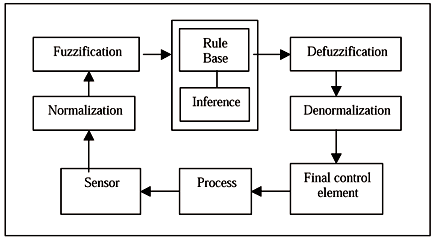
\includegraphics [scale=0.4]{fuzzysystem}
\caption{General Structure of a FLC.}
\end{figure}

The principal functions of a FLC include: \\

\begin{itemize}
\item \textbf{Fuzzifier:} It is responsible for assigning a membership value to each fuzzy set, through the characteristic functions associated to the fuzzy sets. The inputs must be normalized values with concrete values and the outputs are the membership values of each fuzzy set.
\item \textbf{Rule Base:} FLCs use rules, which combine one or many input fuzzy sets (antecedents or premises) and then associate an output fuzzy set (consequent or result). The rules are IF-THEN statements. The input fuzzy sets are associated with fuzzy logic operators (AND,OR,NOT,etc.).
\item \textbf{Fuzzy Inference:} It is the process of formulating the mapping from a given input to an output using fuzzy logic. The process of fuzzy inference involves membership functions, fuzzy logic operators, and IF-THEN rules.
\item \textbf{Defuzzifier:} With the output fuzzy set obtained in the inference engine and through mathematical methods of defuzzification is obtained a concrete value as the output. This value is denormalized to be sent to the plant.
\end{itemize}

Fuzzy logic presents robust and flexible inference methods in problems subject to imprecision and uncertainty. The linguistic representation of knowledge permits a person to interact with a fuzzy system in an easy manner \cite{pawar:fuzzy}.

\subsection{Genetic Fuzzy System (GFS)}

GFSs have been widely employed to solve classification, regression and control problems. The main feature that highlights GFSs in respect to other mathematical, statistical and artificial intelligence models is its capability of extracting knowledge from datasets or industrial plants and state it in linguistic terms with reasonable accuracy\cite{koshiyama:gfs}.

\begin{figure}[h]
\centering
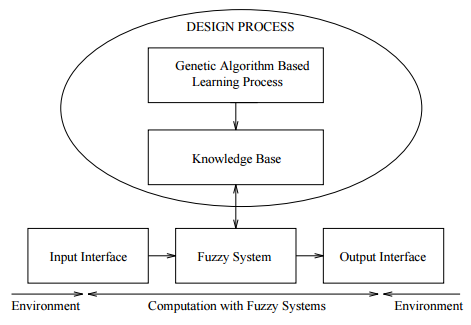
\includegraphics [scale=0.4]{hybridsys}
\caption{General structure of a GFS}
\end{figure}

The principles and operations of EvoNorm and FLCs have been briefly described in the previous sections. These two soft computing tools can be combined to form a GFS in which EvoNorm is used to evolve a fuzzy system by tuning the learning fuzzy rules.

\section{Experimental Results}

\subsection{Design of the plant}

\begin{figure}[h]
\centering
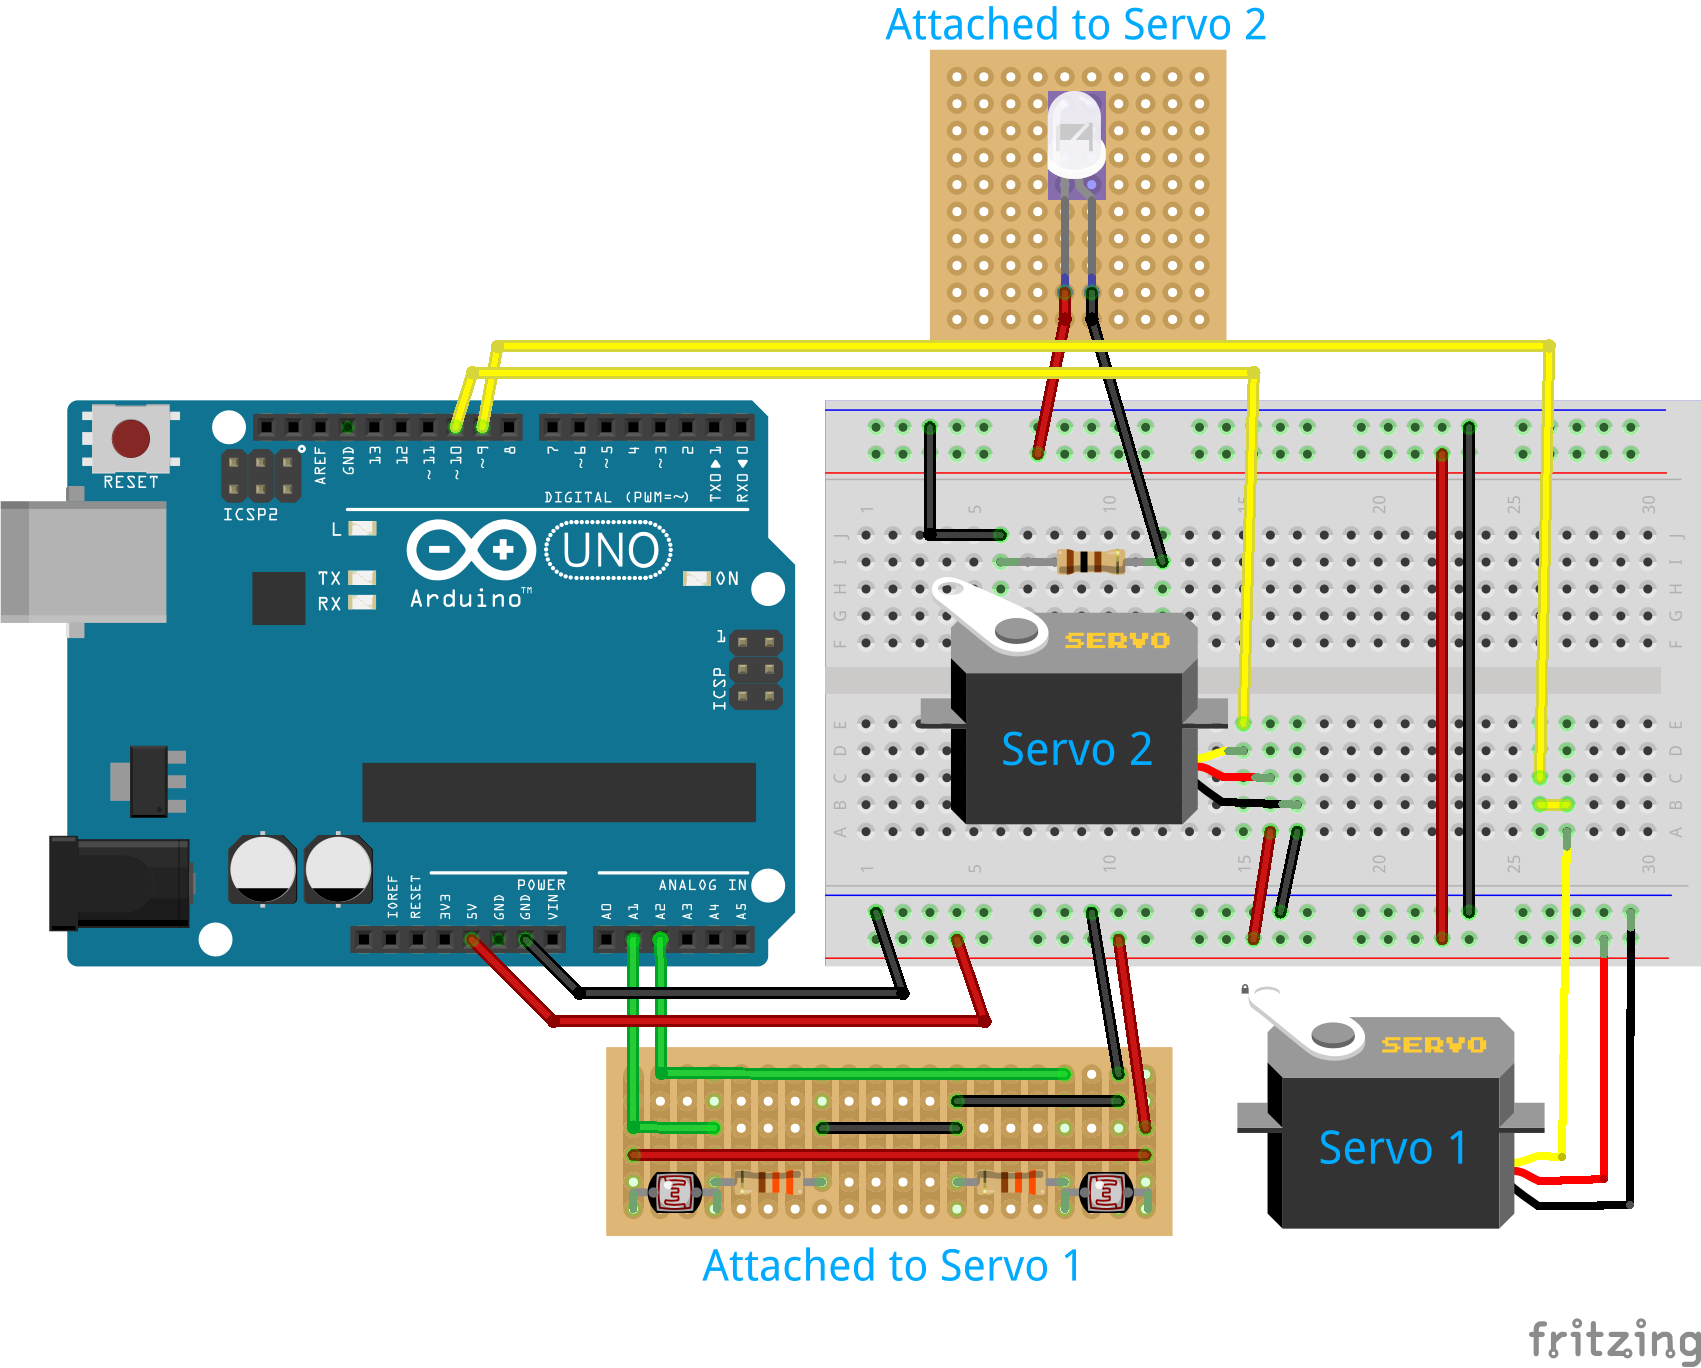
\includegraphics [scale=0.4]{gfsillustration}
\caption{Illustration of the GFS.}
\end{figure}

The hardware of the GFS (illustrated in figure 3) is composed of two inputs and one output. The inputs consist of two LDRs ($Input_1$ and $Input_2$), which have a variable resistance due to light change in the environment. Both LDRs are soldered to a board (end to end) attached to \textit{Servo 1}. A board with an ultrabright LED is attached to a \textit{Servo 2} to make this change of light in the environment more variable. Through a voltage divider the analog input signals are sent to the Arduino board. With the generation of a random population $P$ with $I_p=10$, the consequent of the rules for each combination of input fuzzy sets ($D_r$) are created. The output of the FLC is the angle of the \textit{Servo 1} in the range of 45-135\degree, which will depend on the consequents created and the light sensed by the inputs. The consequents are evaluated by EvoNorm for each individual of the population $P$ through the evaluation function. In this experiment, the evaluation function is $error=|Input_2-Input_1|$. The best individual will be the one in which $error$ is closest to zero. Being $I_s=2$, EvoNorm selects the 2 best individuals and generates a new population through the normal function. The normal function used in the code is based in the Central Limit Theorem Method as stated by Matt Donadio in \cite{donadio:nf}.The EvoNorm algorithm tries to find the optimal solution following the steps (2)-(7) of the frame in section 2.1. For this experiment, the steps (2)-(7) are repeated until 10 generations of new populations have been created.

The schematic diagram of the system is shown in figure 4.

\begin{figure}[h]
\centering
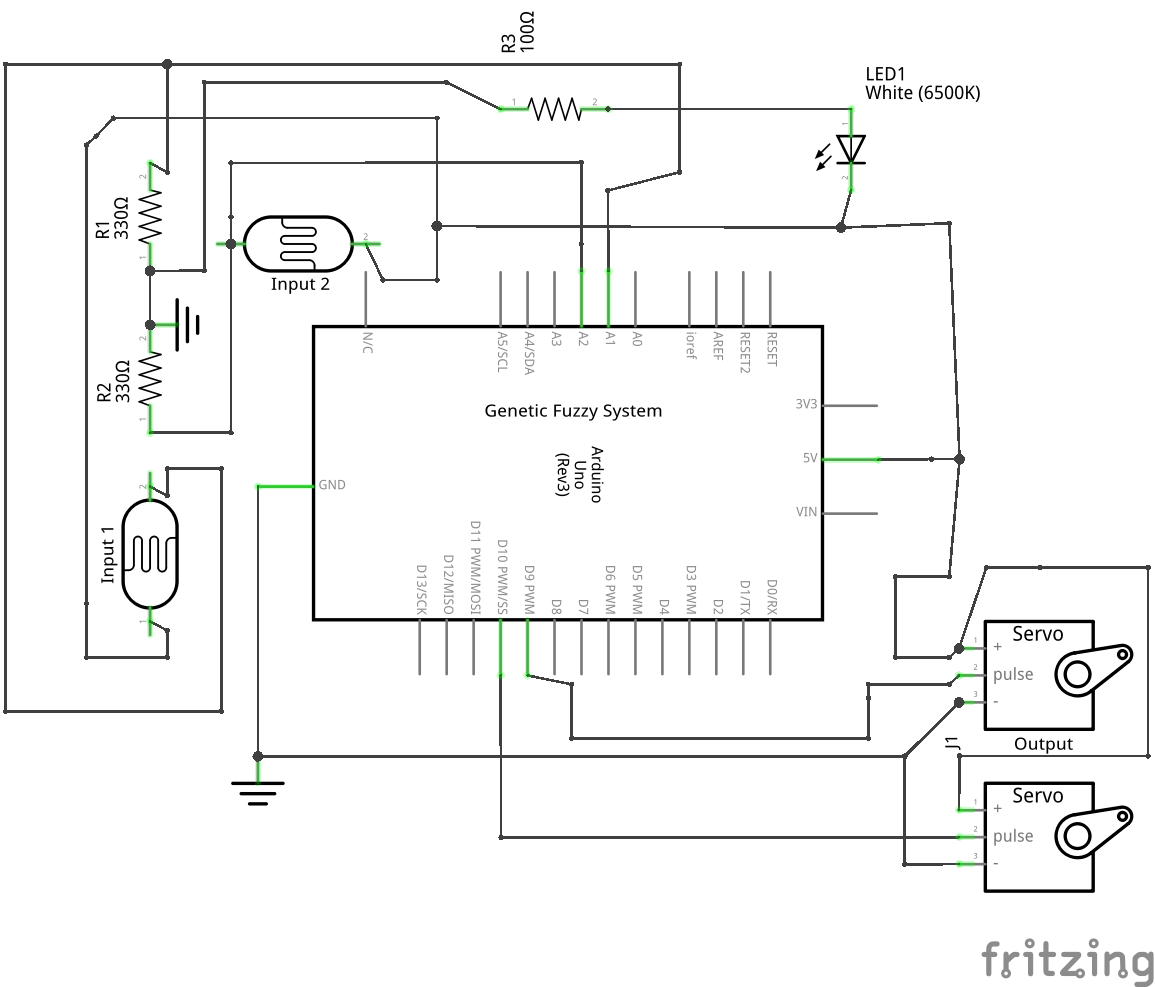
\includegraphics [scale=0.75]{gfsschem}
\caption{Schematic diagram of the GFS.}
\end{figure}

\bigskip
\bigskip

\subsection{Results}

The following results show the evolution of the error of each individual in $P$ through 10 generations. For a better visualization of the results, the evolution of the error is splitted in 2 graphs (Figure 5 and 6).

\begin{figure}[h!]
\centering
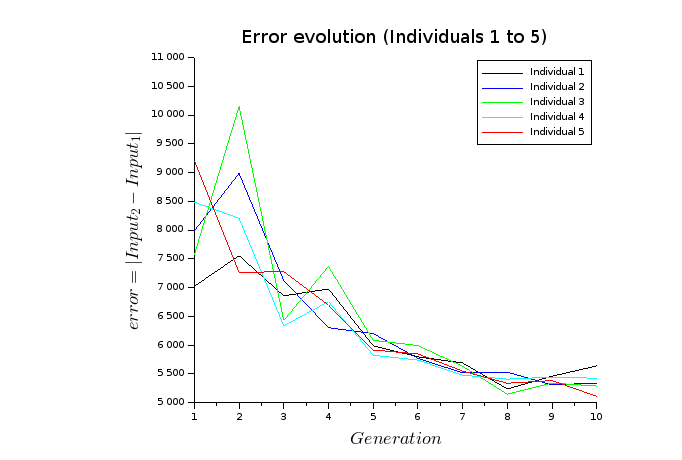
\includegraphics [scale=0.32]{errev1}
\caption{Error evolution (Individuals 1-5).}
\end{figure}

\begin{figure}[h!]
\centering
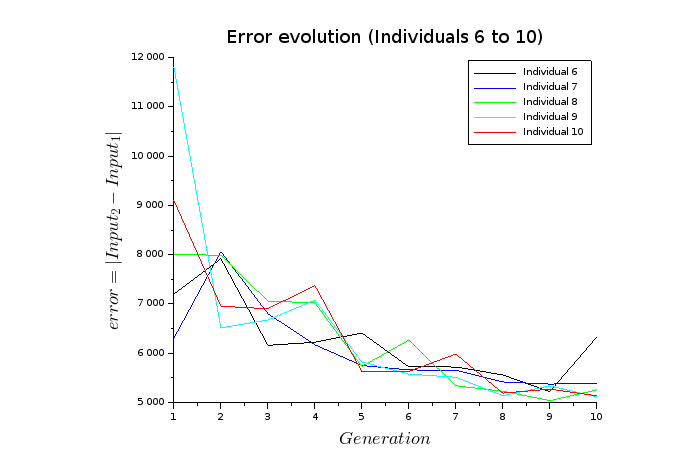
\includegraphics [scale=0.32]{errev2}
\caption{Error evolution (Individuals 6-10).}
\end{figure}

The next graph (figure 7) shows the mean error of the 10 individual. The mean error tends to decrease in each generation (except for the last generation).

\begin{figure}[h!]
\centering
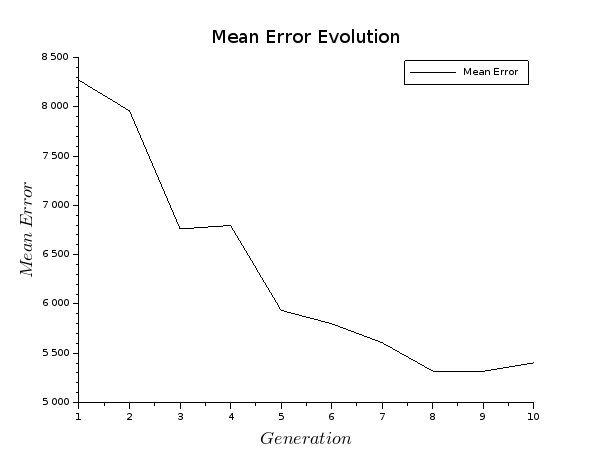
\includegraphics [scale=0.32]{me_evolution}
\caption{Mean Error Evolution.}
\end{figure}

%\begin{table}[h]
%\centering
%\caption{Frequency of Special Characters}
%\begin{tabular}{|c|c|l|} \hline
%Non-English or Math&Frequency&Comments\\ \hline
%\O & 1 in 1,000& For Swedish names\\ \hline
%$\pi$ & 1 in 5& Common in math\\ \hline
%\$ & 4 in 5 & Used in business\\ \hline
%$\Psi^2_1$ & 1 in 40,000& Unexplained usage\\
%\hline\end{tabular}
%\end{table}

%\begin{table*}
%\centering
%\caption{Some Typical Commands}
%\begin{tabular}{|c|c|l|} \hline
%Command&A Number&Comments\\ \hline
%\texttt{{\char'134}alignauthor} & 100& Author alignment\\ \hline
%\texttt{{\char'134}numberofauthors}& 200& Author enumeration\\ \hline
%\texttt{{\char'134}table}& 300 & For tables\\ \hline
%\texttt{{\char'134}table*}& 400& For wider tables\\ \hline\end{tabular}
%\end{table*}
% end the environment with {table*}, NOTE not {table}!

\section{Conclusions}

The results show that is possible to obtain an optimal solution for a FLC with the help of an evolutionary algorithm as EvoNorm. Physically, the operation of the system has an uncertain behavior and the output varies in some cases abruptly; it is supposed that there could be very similar rules in which the consequent is completely different.The minimum mean error has a value of 5316.1, therefore the next step will be to modify the code embedded into the Arduino to obtain better possible solutions by decreasing error in a more substantial way.

%\begin{figure*}
%\centering
%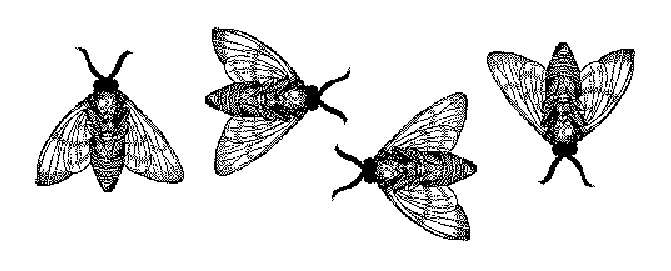
\includegraphics{flies}
%\caption{A sample black and white graphic
%that needs to span two columns of text.}
%\end{figure*}

%
% The following two commands are all you need in the
% initial runs of your .tex file to
% produce the bibliography for the citations in your paper.
\bibliographystyle{abbrv}
\bibliography{sigproc}  % sigproc.bib is the name of the Bibliography in this case

\end{document}
